
\section{Results}
\label{sec:results}

\subsection{Strategy-Dependent Severity}
\label{sec:strategy-severity}

Table~\ref{tab:aggregate-ii} reports the median compound severity difference across strategies and sparsity levels. Under importance-based eviction, $\Delta$ increases from $0.39$ at $s{=}0.15$ to $8.48$ at $s{=}0.30$---a $22{\times}$ amplification (all Bonferroni-corrected $p \ll 10^{-10}$). Random eviction develops a detectable but weak phase gradient above $s \approx 0.20$: at $s \leq 0.20$, $\Delta$ is non-significant ($0.01$--$0.03$; CIs span zero); at $s \geq 0.25$, $\Delta$ becomes significant ($0.26$--$0.51$; $p_{\text{Bonf}} < 0.006$) but $15$--$17{\times}$ smaller than under importance-based eviction. Both strategies exhibit monotonic dose-response (Jonckheere-Terpstra $z{=}6.2$--$33.7$, all $p < 10^{-9}$), but importance masking effect sizes are an order of magnitude larger.

\begin{table}[t]
\centering
\small
\caption{Median of per-problem paired severity differences ($\Delta$) by eviction strategy and sparsity level on DeepSeek-R1-Distill-Qwen-7B ($n{=}496$, MATH-500).}
\label{tab:aggregate-ii}
\begin{tabular}{@{}lcccc@{}}
\toprule
Strategy & $s{=}0.15$ & $s{=}0.20$ & $s{=}0.25$ & $s{=}0.30$ \\
\midrule
Importance & 0.39 & 1.21 & 3.99 & 8.48 \\
Random     & 0.01 & 0.03 & 0.26 & 0.51 \\
\bottomrule
\end{tabular}
\end{table}


\subsection{Phase-Modulated Amplification}
\label{sec:phase-amplification}

Decomposing II by reasoning phase reveals that strategy-dependent severity is driven by amplification in the low-sparsity phase. Table~\ref{tab:main-results} reports the per-phase breakdown. Under importance-based eviction, the median II in the low-sparsity phase rises from $0.357$ ($s{=}0.15$) to $8.456$ ($s{=}0.30$), while the high-sparsity phase remains near zero ($0.003$--$0.038$), yielding paired median differences $\Delta$ from $0.39$ to $8.48$ (all $p \ll 10^{-10}$). Random eviction shows a detectable but much weaker phase gradient at $s \geq 0.25$ ($\Delta{=}0.26$--$0.51$; $p_{\text{Bonf}} < 0.006$), $15$--$17{\times}$ smaller than importance-based at matched sparsity. Figure~\ref{fig:hero} visualizes the dose-response relationship for both models. The per-problem amplification ratio $G$ (Eq.~\ref{eq:gradient}) provides an auxiliary illustrative perspective and is reported in Appendix~\ref{app:g-metric}.
Under the multiplicative null ($r_b = r_a \cdot r_k$; Appendix~\ref{app:multiplicative-null}), the phase-severity gradient is preserved ($G_{\times}{=}21$--$64{\times}$); we report additive-null values throughout as the more conservative estimates.

\begin{table*}[t]
\centering
\small
\caption{Per-phase interaction index (II) at $n{=}496$/$475$. $\Delta{=}\widetilde{\mathrm{II}^{(i)}_{\textit{low}} - \mathrm{II}^{(i)}_{\textit{high}}}$: median of per-problem paired differences (not the difference of column medians) with bootstrap 95\% CI ($B{=}10{,}000$). $G$ values reported in Appendix~\ref{app:g-metric}. Profiling-subset values ($n{=}50$) in Table~\ref{tab:profiling-subset}.}
\label{tab:main-results}
\begin{tabular}{@{}llcccc@{}}
\toprule
$s$ & Strategy & $\widetilde{\mathrm{II}}_{\textit{high}}$ & $\widetilde{\mathrm{II}}_{\textit{low}}$ & $\Delta$\; [95\% CI] & $p_{\text{Bonf}}$ \\
\midrule
\multicolumn{6}{@{}l}{\textit{DeepSeek-R1-Distill-Qwen-7B ($n{=}496$)}} \\
0.15 & Importance & 0.003 & 0.357 & 0.39\; $[0.35,\; 0.44]$ & $< 10^{-10}$ \\
0.15 & Random     & 0.083 & 0.090 & 0.01\; $[-0.02,\; 0.04]$ & ns \\
\addlinespace
0.20 & Importance & 0.008 & 1.211 & 1.21\; $[1.11,\; 1.34]$ & $< 10^{-10}$ \\
0.20 & Random     & 0.270 & 0.357 & 0.03\; $[-0.01,\; 0.08]$ & ns \\
\addlinespace
0.25 & Importance & 0.021 & 3.971 & 3.99\; $[3.53,\; 4.36]$ & $< 10^{-10}$ \\
0.25 & Random     & 1.113 & 1.514 & 0.26\; $[0.13,\; 0.35]$ & $< 0.006$ \\
\addlinespace
0.30 & Importance & 0.038 & 8.456 & 8.48\; $[7.75,\; 9.69]$ & $< 10^{-10}$ \\
0.30 & Random     & 3.112 & 3.848 & 0.51\; $[0.26,\; 0.89]$ & $< 0.006$ \\
\midrule
\multicolumn{6}{@{}l}{\textit{Qwen2.5-7B-Instruct ($n{=}475$)}} \\
0.15 & Importance & $-$0.000$^{\ddagger}$ & 0.044 & 0.07\; $[0.05,\; 0.09]$ & $< 10^{-14}$ \\
0.15 & Random     & 0.094 & 0.097 & $-$0.01\; $[-0.04,\; 0.01]$ & ns \\
\addlinespace
0.20 & Importance & 0.000 & 0.275 & 0.31\; $[0.26,\; 0.36]$ & $< 10^{-14}$ \\
0.20 & Random     & 0.291 & 0.356 & 0.02\; $[-0.01,\; 0.07]$ & ns \\
\addlinespace
0.25 & Importance & 0.004 & 1.053 & 1.07\; $[0.98,\; 1.18]$ & $< 10^{-14}$ \\
0.25 & Random     & 1.108 & 1.769 & 0.39\; $[0.24,\; 0.55]$ & $< 10^{-10}$ \\
\addlinespace
0.30 & Importance & 0.014 & 3.208 & 3.16\; $[2.78,\; 3.56]$ & $< 10^{-14}$ \\
0.30 & Random     & 2.819 & 4.253 & 0.91\; $[0.61,\; 1.26]$ & $< 10^{-13}$ \\
\bottomrule
\multicolumn{6}{@{}p{0.92\textwidth}}{\footnotesize $^{\ddagger}$ Negative II at this sparsity reflects \texttt{bfloat16} numerical noise when the interaction effect approaches zero ($|\mathrm{II}| < 10^{-4}$). $\Delta{=}0.07$, $p{=}8.7 \times 10^{-15}$ supports $\mathrm{II}_{\textit{low}} > \mathrm{II}_{\textit{high}}$.}
\end{tabular}
\end{table*}

\begin{figure*}[t]
\centering
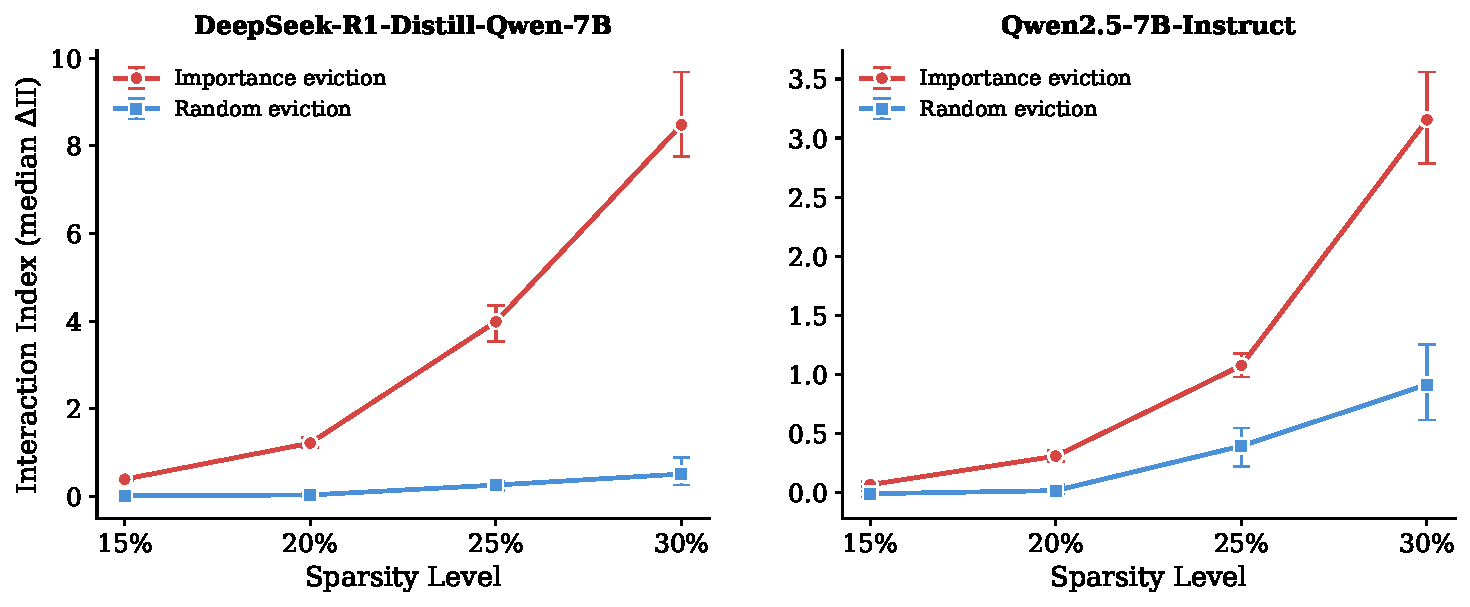
\includegraphics[width=\textwidth]{fig1_ii_scatter.pdf}
\caption{Paired median difference $\Delta$ (primary metric) as a function of sparsity level $s$ for DeepSeek-R1-Distill-Qwen-7B ($n{=}496$, left) and Qwen2.5-7B-Instruct ($n{=}475$, right). Importance-based eviction (red) exhibits monotonically increasing $\Delta$ ($0.39$--$8.48$ for DeepSeek, $0.07$--$3.16$ for Qwen); random eviction (blue) remains near zero at low sparsity (ns) and shows weak effects at $s \geq 0.25$. Error bars show asymmetric bootstrap 95\% CIs. DeepSeek importance effects are ${\sim}2.7{\times}$ larger than Qwen, consistent with the training-paradigm contrast (\S\ref{sec:cross-model}). Significance: {*}{*}{*}\,$p_{\text{Bonf}} < 0.001$; {*}{*}\,$p_{\text{Bonf}} < 0.01$; ns\,$p_{\text{Bonf}} > 0.05$.}
\label{fig:hero}
\end{figure*}


\subsection{Phase-Strategy Crossover}
\label{sec:crossover}

The phase-strategy crossover is model-dependent. For DeepSeek ($n{=}496$), a strategy ranking reversal emerges at all four sparsity levels: at $s{=}0.25$, importance-based eviction yields \emph{lower} II than random in the high-sparsity phase ($0.021$ vs.\ $1.113$) but \emph{higher} II in the low-sparsity phase ($3.971$ vs.\ $1.514$---a $2.6{\times}$ reversal; both $p < 10^{-4}$), with reversal magnitude ranging from $2.2{\times}$ to $4.0{\times}$ across $s \in \{0.15, 0.20, 0.25, 0.30\}$. Qwen does \emph{not} exhibit this crossover: importance-based eviction produces lower II than random in both phases (e.g., at $s{=}0.25$: high $0.004$ vs.\ $1.108$; low $1.053$ vs.\ $1.769$). This divergence suggests the crossover arises from model-specific attention head specialization patterns rather than a universal compound-sparsity property. Full crossover analysis appears in Appendix~\ref{app:crossover-details}.

\subsection{Replication Across Training Paradigms}
\label{sec:cross-model}

DeepSeek-R1-Distill-Qwen-7B (distillation-trained) and Qwen2.5-7B-Instruct (instruction-tuned) share the Qwen2 backbone but differ in training objective, providing a within-architecture-family comparison across training paradigms.
Qwen2.5-7B-Instruct ($n_{\text{eff}}{=}475$) reproduces the monotonic severity gradient: $\Delta$ increases from $0.07$ at $s{=}0.15$ to $3.16$ at $s{=}0.30$ (all Bonferroni-corrected $p < 10^{-14}$), paralleling DeepSeek at approximately one-quarter to one-sixth the magnitude. Both models yield strictly increasing median $\Delta$ trajectories (Jonckheere-Terpstra $z \geq 6.2$, $p < 10^{-9}$; see \S\ref{par:stats}). Random eviction on Qwen mirrors DeepSeek: non-significant at $s \leq 0.20$, becoming significant at $s \geq 0.25$ ($\Delta{=}0.39$--$0.91$; $p_{\text{Bonf}} < 10^{-10}$) but $2.7$--$3.5{\times}$ weaker than importance-based. A caveat: 45.2\% of Qwen problems yield null mid-phase segments due to low temporal autocorrelation ($r{=}0.718$ vs.\ $0.894$); this does not affect $\Delta$ (Appendix~\ref{app:qwen-null-rate}). Full tables in Appendix~\ref{app:cross-model-details}.

\subsection{Cross-Architecture Validation}
\label{sec:cross-arch}

Cross-architecture validation on DeepSeek-R1-Distill-Llama-8B (LlamaForCausalLM, $n{=}250$, MATH-500) supports the generality of phase-modulated compound interaction beyond the Qwen2 architecture family. Under importance-based eviction, the paired median difference $\Delta$ rises monotonically from $0.050$ ($s{=}0.15$) to $0.695$ ($s{=}0.30$), with large effect sizes throughout ($d_z{=}0.81$--$1.15$; all $p < 10^{-29}$; Table~\ref{tab:llama-cross-arch}).

A key architectural difference emerges in strategy specificity. On LLaMA, random eviction also exhibits significant phase gradients ($\Delta{=}0.025$--$0.271$; $d_z{=}0.41$--$0.46$; all $p < 10^{-12}$), unlike DeepSeek and Qwen where random is non-significant at $s \leq 0.20$. The importance/random $\Delta$ ratio is $2.0$--$2.6{\times}$ on LLaMA, substantially weaker than the $15$--$17{\times}$ observed on DeepSeek. Dose-response monotonicity holds for both strategies (all conditions monotonic). This indicates that the phase gradient itself is architecture-general, while the degree of strategy specificity is architecture-dependent, likely reflecting differences between GQA (LLaMA, 32 heads with 8 KV groups) and MHA (Qwen2, 28 heads) in how head pruning differentially disrupts importance scoring.

Absolute interaction magnitudes are approximately $7$--$12{\times}$ smaller than Qwen2-family models at matched sparsity, consistent with architecture-specific attention head specialization patterns. Full per-condition breakdowns appear in Appendix~\ref{app:cross-arch}.

\subsection{Scoring-Independent Control}
\label{sec:scoring-control}

To distinguish whether the phase gradient arises from attention-score-based eviction dynamics or from token removal \emph{per se} under compound sparsity, we introduce a scoring-independent control: \emph{recency eviction}, which removes the oldest non-BOS positions regardless of attention scores. This eliminates the feedback loop between head pruning and importance scoring while maintaining identical compression ratios.

On DeepSeek ($n{=}100$, MATH-500), recency eviction produces a negative or absent phase gradient across $s \in \{0.15, 0.25\}$: $\Delta{=}-0.013$ (CI spans zero, NS) at $s{=}0.15$ and $\Delta{=}-0.091$ (CI excludes zero, significantly \emph{negative}) at $s{=}0.25$. Both contrast sharply with importance-based eviction at matched sparsity ($\Delta{=}+0.39$ and $+3.99$; all $p < 10^{-69}$). At $s{=}0.30$, KV perplexity saturation (${>}10^5$) under recency eviction renders per-segment II numerically unreliable; the gradient estimate ($+0.112$) is non-significant (CI $[-0.01,\; +0.46]$, spans zero).

This triangulation across three eviction strategies provides strong evidence for mechanism discrimination:
\begin{itemize}[nosep,leftmargin=*]
    \item \textbf{Importance}: super-additive compound interaction ($\mathrm{II} > 0$) with large positive phase gradient ($\Delta$: $+0.39$ to $+8.48$)
    \item \textbf{Random}: super-additive interaction ($\mathrm{II} > 0$) with near-zero phase gradient ($\Delta \approx 0$ at $s \leq 0.20$)
    \item \textbf{Recency}: sub-additive/zero interaction ($\mathrm{II} \leq 0$) with absent or negative phase gradient ($\Delta \leq 0$ at $s \leq 0.25$; NS at $s{=}0.30$)
\end{itemize}
The recency control rules out two alternative explanations: (1)~the phase gradient is not a segmentation artifact, since the same phase boundaries produce no positive gradient under recency eviction; (2)~the gradient is not an inherent property of removing tokens under compound sparsity, since recency removes the same fraction of tokens without producing phase-dependent severity. Phase-dependent compound severity is specifically driven by attention-score-based selection, as evidenced by its absence under both position-based and random controls.

\subsection{Scale Analysis: Qwen2.5-14B}
\label{sec:scale-14b}

To assess whether phase-modulated severity persists at larger model scale within the same architecture family, we evaluate Qwen2.5-14B-Instruct on MATH-500 ($n{=}500$) at $s \in \{0.15, 0.20, 0.25, 0.30\}$.

\begin{table}[t]
\centering
\small
\caption{Median of per-problem paired severity differences ($\Delta$) under importance-based eviction on Qwen2.5-14B-Instruct (MATH-500). \textit{Results pending.}}
\label{tab:scale-14b}
\begin{tabular}{@{}lcccc@{}}
\toprule
Strategy & $s{=}0.15$ & $s{=}0.20$ & $s{=}0.25$ & $s{=}0.30$ \\
\midrule
Importance & --- & --- & --- & --- \\
Random     & --- & --- & --- & --- \\
\bottomrule
\end{tabular}
\end{table}

%% PLACEHOLDER: Fill Table~\ref{tab:scale-14b} when c12 experiment completes.
%% Expected analysis: (1) whether 14B amplifies or attenuates severity relative to 7B,
%% (2) whether strategy specificity ratio is scale-invariant,
%% (3) comparison of phase segmentation thresholds at larger scale.

\subsection{Cross-Benchmark Validation: GSM8K}
\label{sec:cross-benchmark}

To assess task generalization, we evaluate both models on GSM8K ($n{=}50$) at $s \in \{0.15, 0.20, 0.25, 0.30\}$. On DeepSeek (clean data, no output truncation), importance-based eviction replicates the MATH-500 phase gradient across all four sparsity levels with a strict dose-response: $\Delta{=}0.24$ at $s{=}0.15$ rising to $4.68$ at $s{=}0.30$ (all $p \leq 0.0003$, Wilcoxon). Strategy specificity on GSM8K manifests as a \emph{qualitative} gap: importance-based eviction produces significant phase gradients while random eviction is non-significant across all conditions (CIs spanning zero).

We interpret this attenuation as \emph{reasoning depth scaling}: strategy specificity scales with reasoning chain depth. MATH-500 (complex multi-step reasoning, strategy ratio $15$--$17{\times}$) produces stronger phase contrast than GSM8K (simpler arithmetic, ratio ${\sim}2{\times}$ from point estimates). Within MATH-500, longer traces exhibit higher strategy specificity (Spearman $\rho > 0$, $p < 0.02$), providing continuous correlational support. This scaling relationship is predictive: tasks with deeper reasoning chains should exhibit stronger strategy${\times}$phase interactions, because longer low-sparsity phases provide more opportunity for importance discrimination collapse to accumulate. Qwen GSM8K results are inconclusive due to generation truncation (\texttt{max\_new\_tokens}${=}$2047): while directional consistency holds at $s \geq 0.25$ ($\Delta{=}1.14$--$4.62$; $p < 10^{-4}$), absolute values and phase assignments are unreliable because all outputs hit the token limit. Full tables in Appendix~\ref{app:gsm8k}.

\paragraph{GSM8K accuracy under compound sparsity.}
A power analysis on GSM8K ($n{=}50$) reveals a strategy-dependent asymmetry in downstream accuracy. Under random head removal, all 8 conditions (2 models $\times$ 4 sparsity levels) are non-significant (max $|d|{=}0.164$). Post-hoc power analysis indicates $n{=}50$ can detect effects of $d \geq 0.40$ ($\alpha{=}0.05$, power${=}0.80$); all random conditions showed $|d| \leq 0.164$, meaning the null results may reflect insufficient power rather than true absence of effect. Under importance-based pruning, Qwen exhibits a medium-sized accuracy degradation at $s \geq 0.25$ ($d \approx 0.63$, power ${>}\,0.99$), consistent with the PPL-based severity gradient observed on MATH-500. DeepSeek importance conditions exhibit a qualitative downward trend in accuracy but are excluded from parametric inference due to heavy-tailed distributions that violate test assumptions.

\subsection{Cross-Benchmark Validation: GPQA Diamond}
\label{sec:cross-benchmark-gpqa}

To assess generalization beyond mathematical reasoning, we evaluate both models on GPQA Diamond~\cite{rein-gpqa-2024} ($n{=}198$), a graduate-level science QA benchmark requiring multi-step reasoning across physics, chemistry, and biology.

\begin{table}[t]
\centering
\small
\caption{Median of per-problem paired severity differences ($\Delta$) under importance-based eviction on GPQA Diamond. \textit{Results pending.}}
\label{tab:gpqa-results}
\begin{tabular}{@{}lcccc@{}}
\toprule
Model & $s{=}0.15$ & $s{=}0.20$ & $s{=}0.25$ & $s{=}0.30$ \\
\midrule
DeepSeek-R1-Distill-Qwen-7B & --- & --- & --- & --- \\
Qwen2.5-7B-Instruct         & --- & --- & --- & --- \\
\bottomrule
\end{tabular}
\end{table}

%% PLACEHOLDER: Fill Table~\ref{tab:gpqa-results} when c11 experiment completes.
%% Expected analysis: (1) phase gradient direction consistency with MATH-500/GSM8K,
%% (2) strategy specificity comparison across task types (math vs. science reasoning),
%% (3) whether cognitive load modulation hypothesis extends to non-mathematical domains.

\subsection{Statistical Validation}
\label{sec:stat-validation}

Table~\ref{tab:cohens-d} reports the paired median difference $\Delta$ under importance-based eviction for both models at $n{=}496$/$475$. All eight conditions yield CIs excluding zero; within-importance dose-response $d_z$ (s015 vs.\ s030) is $0.94$ (DeepSeek) and $0.92$ (Qwen), both large effects. Importance-based eviction produces significantly larger phase gradients than random at all four sparsity levels ($p_{\text{Bonf}} \ll 10^{-10}$, Wilcoxon; permutation tests in Appendix~\ref{app:permutation-details}).

\begin{table}[t]
\centering
\small
\caption{Median of paired differences ($\Delta_i = \mathrm{II}^{(i)}_{\textit{low}} - \mathrm{II}^{(i)}_{\textit{high}}$) under importance-based eviction with bootstrap 95\% CIs ($B{=}10{,}000$).}
\label{tab:cohens-d}
\begin{tabular}{@{}lcc@{}}
\toprule
$s$ & DS ($n{=}496$): $\widetilde{\Delta}$\; [95\% CI] & QW ($n{=}475$): $\widetilde{\Delta}$\; [95\% CI] \\
\midrule
0.15 & $0.39$\; $[0.35,\; 0.44]$ & $0.07$\; $[0.05,\; 0.09]$ \\
0.20 & $1.21$\; $[1.11,\; 1.34]$ & $0.31$\; $[0.26,\; 0.36]$ \\
0.25 & $3.99$\; $[3.53,\; 4.36]$ & $1.07$\; $[0.98,\; 1.18]$ \\
0.30 & $8.48$\; $[7.75,\; 9.69]$ & $3.16$\; $[2.78,\; 3.56]$ \\
\bottomrule
\multicolumn{3}{@{}l}{\footnotesize All $p_{\text{Bonf}} < 10^{-13}$. Within-importance $d_z$ (s015 vs.\ s030): DS $0.94$, QW $0.92$.}
\end{tabular}
\end{table}

\subsection{Answer-Region Analysis}
\label{sec:answer-region}

Across both models, 93.2\% of answer tokens (\verb|\boxed{}| markers) fall within the high-sparsity phase, where compound interaction is minimal. This non-uniformity identifies \emph{where} severity concentrates: reasoning-trace tokens show $5.7$--$43.5{\times}$ PPL degradation vs.\ $1.3$--$5.3{\times}$ for answer tokens (Wilcoxon $p < 0.001$). However, reasoning-trace degradation may produce \emph{silent reasoning errors}---correct formatting with corrupted intermediate logic \cite{lanham-2023-faithfulness, turpin-2023-biased-cot}---a failure mode that PPL detects but answer-level accuracy may miss.

\subsection{Downstream Accuracy Validation}
\label{sec:accuracy-validation}

To validate that the PPL-based severity gradient translates to downstream task performance, we evaluate MATH-500 accuracy under compound sparsity (importance-based eviction, \texttt{max\_new\_tokens}${=}$8192; Table~\ref{tab:accuracy}). Qwen's minimal truncation ($\leq 4\%$) provides a clean PPL-accuracy bridge.
Qwen ($n{=}100$; truncation $\leq 4\%$) shows gradual decline from $46\%$ (dense) through $s{=}0.25$ ($\delta{=}-4$ to $-13$\,pp) with a sharp cliff at $s{=}0.30$ ($19\%$, $\delta{=}-27$\,pp). DeepSeek ($n{=}50$) degrades more steeply ($74\% \to 4\%$) with a dual-regime structure: at $s \leq 0.20$, degradation is primarily truncation-driven (non-truncated accuracy remains $68$--$71\%$ at $s{=}0.15$--$0.20$ vs.\ $88\%$ dense); at $s \geq 0.25$, both truncation and reasoning quality collapse simultaneously (Appendix~\ref{app:accuracy-details}).
The two models exhibit distinct failure modes reflecting training-paradigm dependence: DeepSeek failures are \emph{truncation-dominated} (truncation $16\% \to 76\%$), while Qwen failures are \emph{wrong-answer-dominated} (truncation $\leq 4\%$, reasoning quality degrades directly). Given minimal truncation, Qwen accuracy data provide a reliable PPL-accuracy bridge; DeepSeek accuracy results, confounded by truncation rates of $16\%$--$76\%$, should be interpreted as qualitative observations only.

We provide a correlational mechanistic analysis in terms of importance discrimination collapse in \S\ref{sec:analysis}.
